%%%%%%%%%%%%%%%%%%%%%%%%%%%%%%%%%%%%%%%%%%%%%%%%%%%%%%%%%%%%%%%%%%%%%%%%%%%%%%%

\section*{\large Exercício 3 - Repita o exercício anterior considerando, entretanto, o algoritmo pmodel.py}
\addcontentsline{toc}{chapter}{\protect\numberline{}\large Exercício 3}%

Os resultados das análises dos sinais referentes a este exercício se encontram na pasta \textbf{Exercise3}. Os valores de $\rho$ da família pmnoise foram .18, .23, .28, .32, .37 e .42, onde os três primeiros representam uma série exógena (com parâmetro $\beta$ = 0.7), e os três últimos representam uma série endógena (com parâmetro $\beta$ = 0.4). Todas as séries foram geradas com tamanho igual a 8192. Os plots abaixo ilustram alguns dos resultados para a série exógena e endógena, respectivamente.

\begin{figure}[ht!]
	%\caption{Série e histogramas.}
	\vspace{0mm}	% acrescentar o espaçamento vertical apropriado entre o título e a borda superior da figura
	\begin{center}
		\resizebox{16cm}{!}{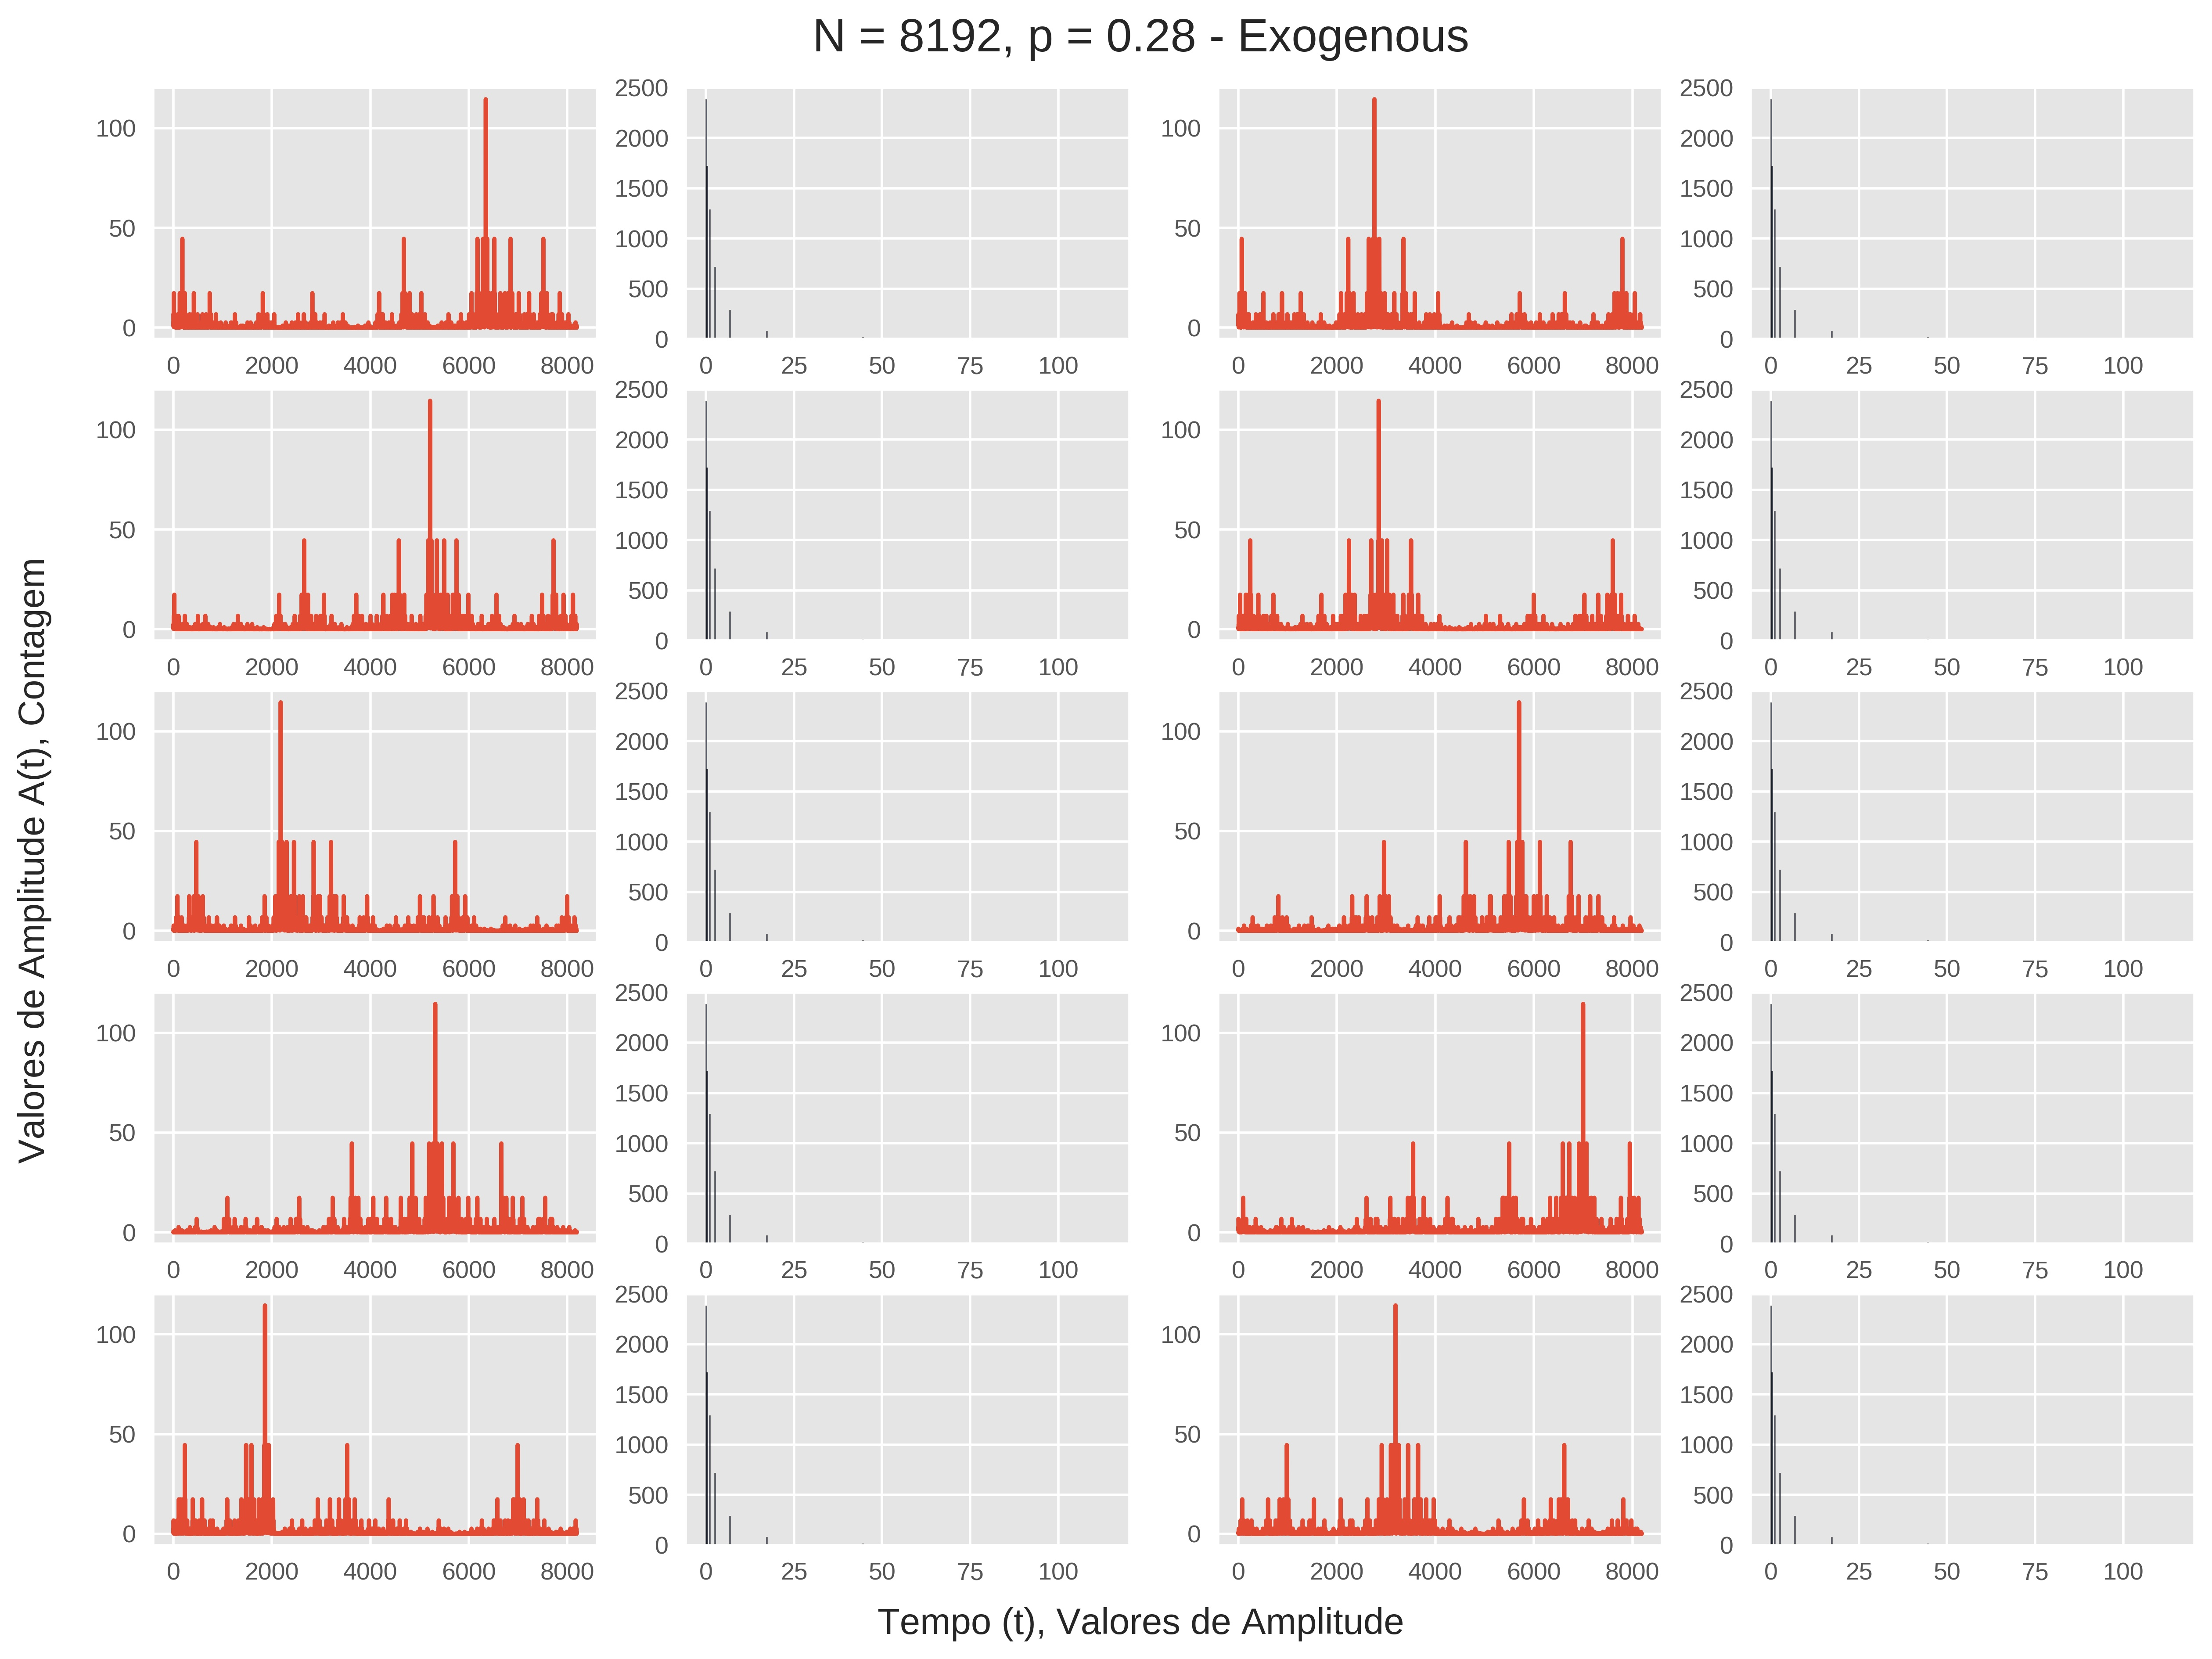
\includegraphics{Figuras/ex3/Exercicio3_p_0.28.jpg}}		
	\end{center}
	\vspace{-2mm}	% acrescentar o espaçamento vertical apropriado entre a borda inferior da figura e a legenda ou a fonte quando não há legenda (o valor pode ser negativo para subir)
	\legenda{Figura 3.1: Plots de 10 sinais da séire exógena ($\beta$ = 0.7) da família pmnoise e seus respectivos histogramas.}	% legenda - para deixar sem legenda usar comando \legenda{} (nunca deve-se comentar o comando \legenda)
	\label{ex3_fig1}
	%\FONTE{}	% fonte consultada (elemento obrigatório, mesmo que seja produção do próprio autor)
\end{figure}

\clearpage

\begin{figure}[ht!]
	%\caption{Série e histogramas.}
	\vspace{0mm}	% acrescentar o espaçamento vertical apropriado entre o título e a borda superior da figura
	\begin{center}
		\resizebox{16cm}{!}{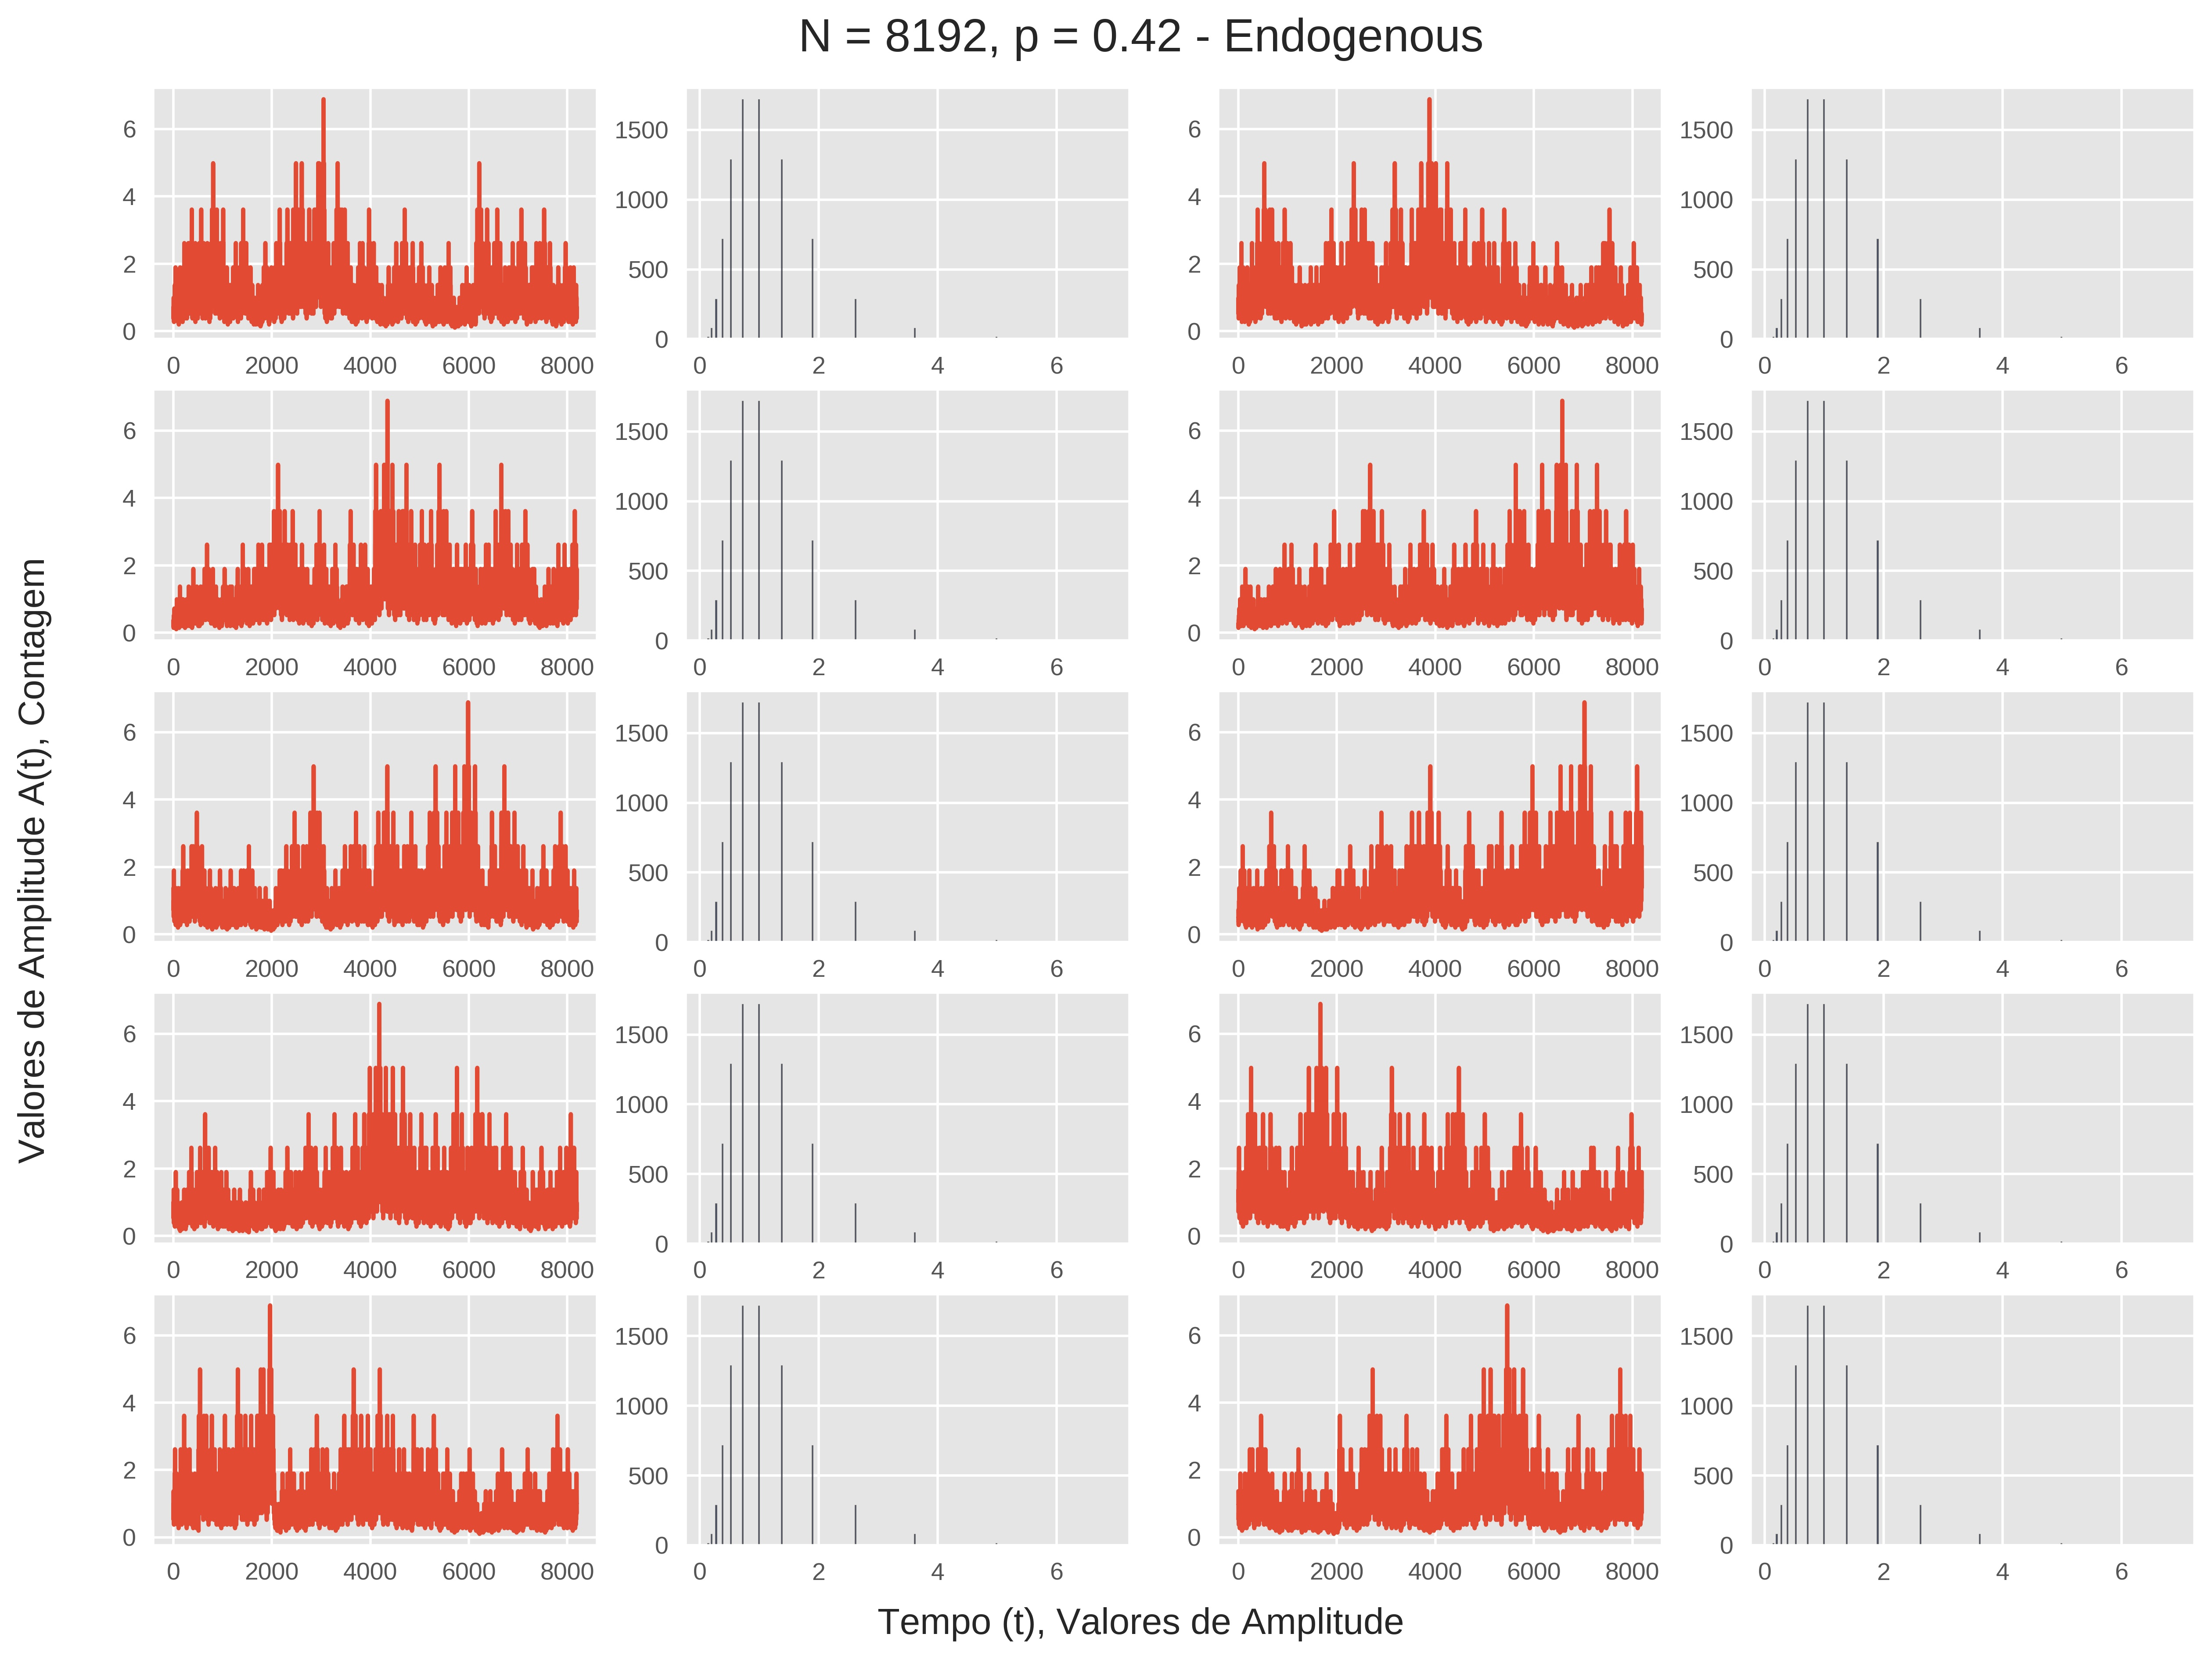
\includegraphics{Figuras/ex3/Exercicio3_p_0.42.jpg}}		
	\end{center}
	\vspace{-2mm}	% acrescentar o espaçamento vertical apropriado entre a borda inferior da figura e a legenda ou a fonte quando não há legenda (o valor pode ser negativo para subir)
	\legenda{Figura 3.2: Plots de 10 sinais da séire endógena ($\beta$ = 0.4) da família pmnoise e seus respectivos histogramas.}	% legenda - para deixar sem legenda usar comando \legenda{} (nunca deve-se comentar o comando \legenda)
	\label{ex3_fig2}
	%\FONTE{}	% fonte consultada (elemento obrigatório, mesmo que seja produção do próprio autor)
\end{figure}

Assim como para as famílias anteriores, a família pmnoise conta com os arquivos \textit{Exercicio3\_momentos.csv},  \textit{Exercicio3\_parametros.csv} e \textit{Exercicio3\_kmeans.csv} em sua pasta, compondo o resultado da análise estatística em conjunto com os demais plots. Abaixo estão os resultados do agrupamento no espaço via kmeans. Fica evidente que há pouca variabilidade de cada sinal no espaço de parâmetros usado, de forma que o agrupamento não permite a caracterização de classes do grupo pmnoise no espaço composto por variância, skewness e kurtosis.

\begin{figure}[ht!]
	%\caption{Série e histogramas.}
	\vspace{0mm}	% acrescentar o espaçamento vertical apropriado entre o título e a borda superior da figura
	\begin{center}
		\resizebox{16cm}{!}{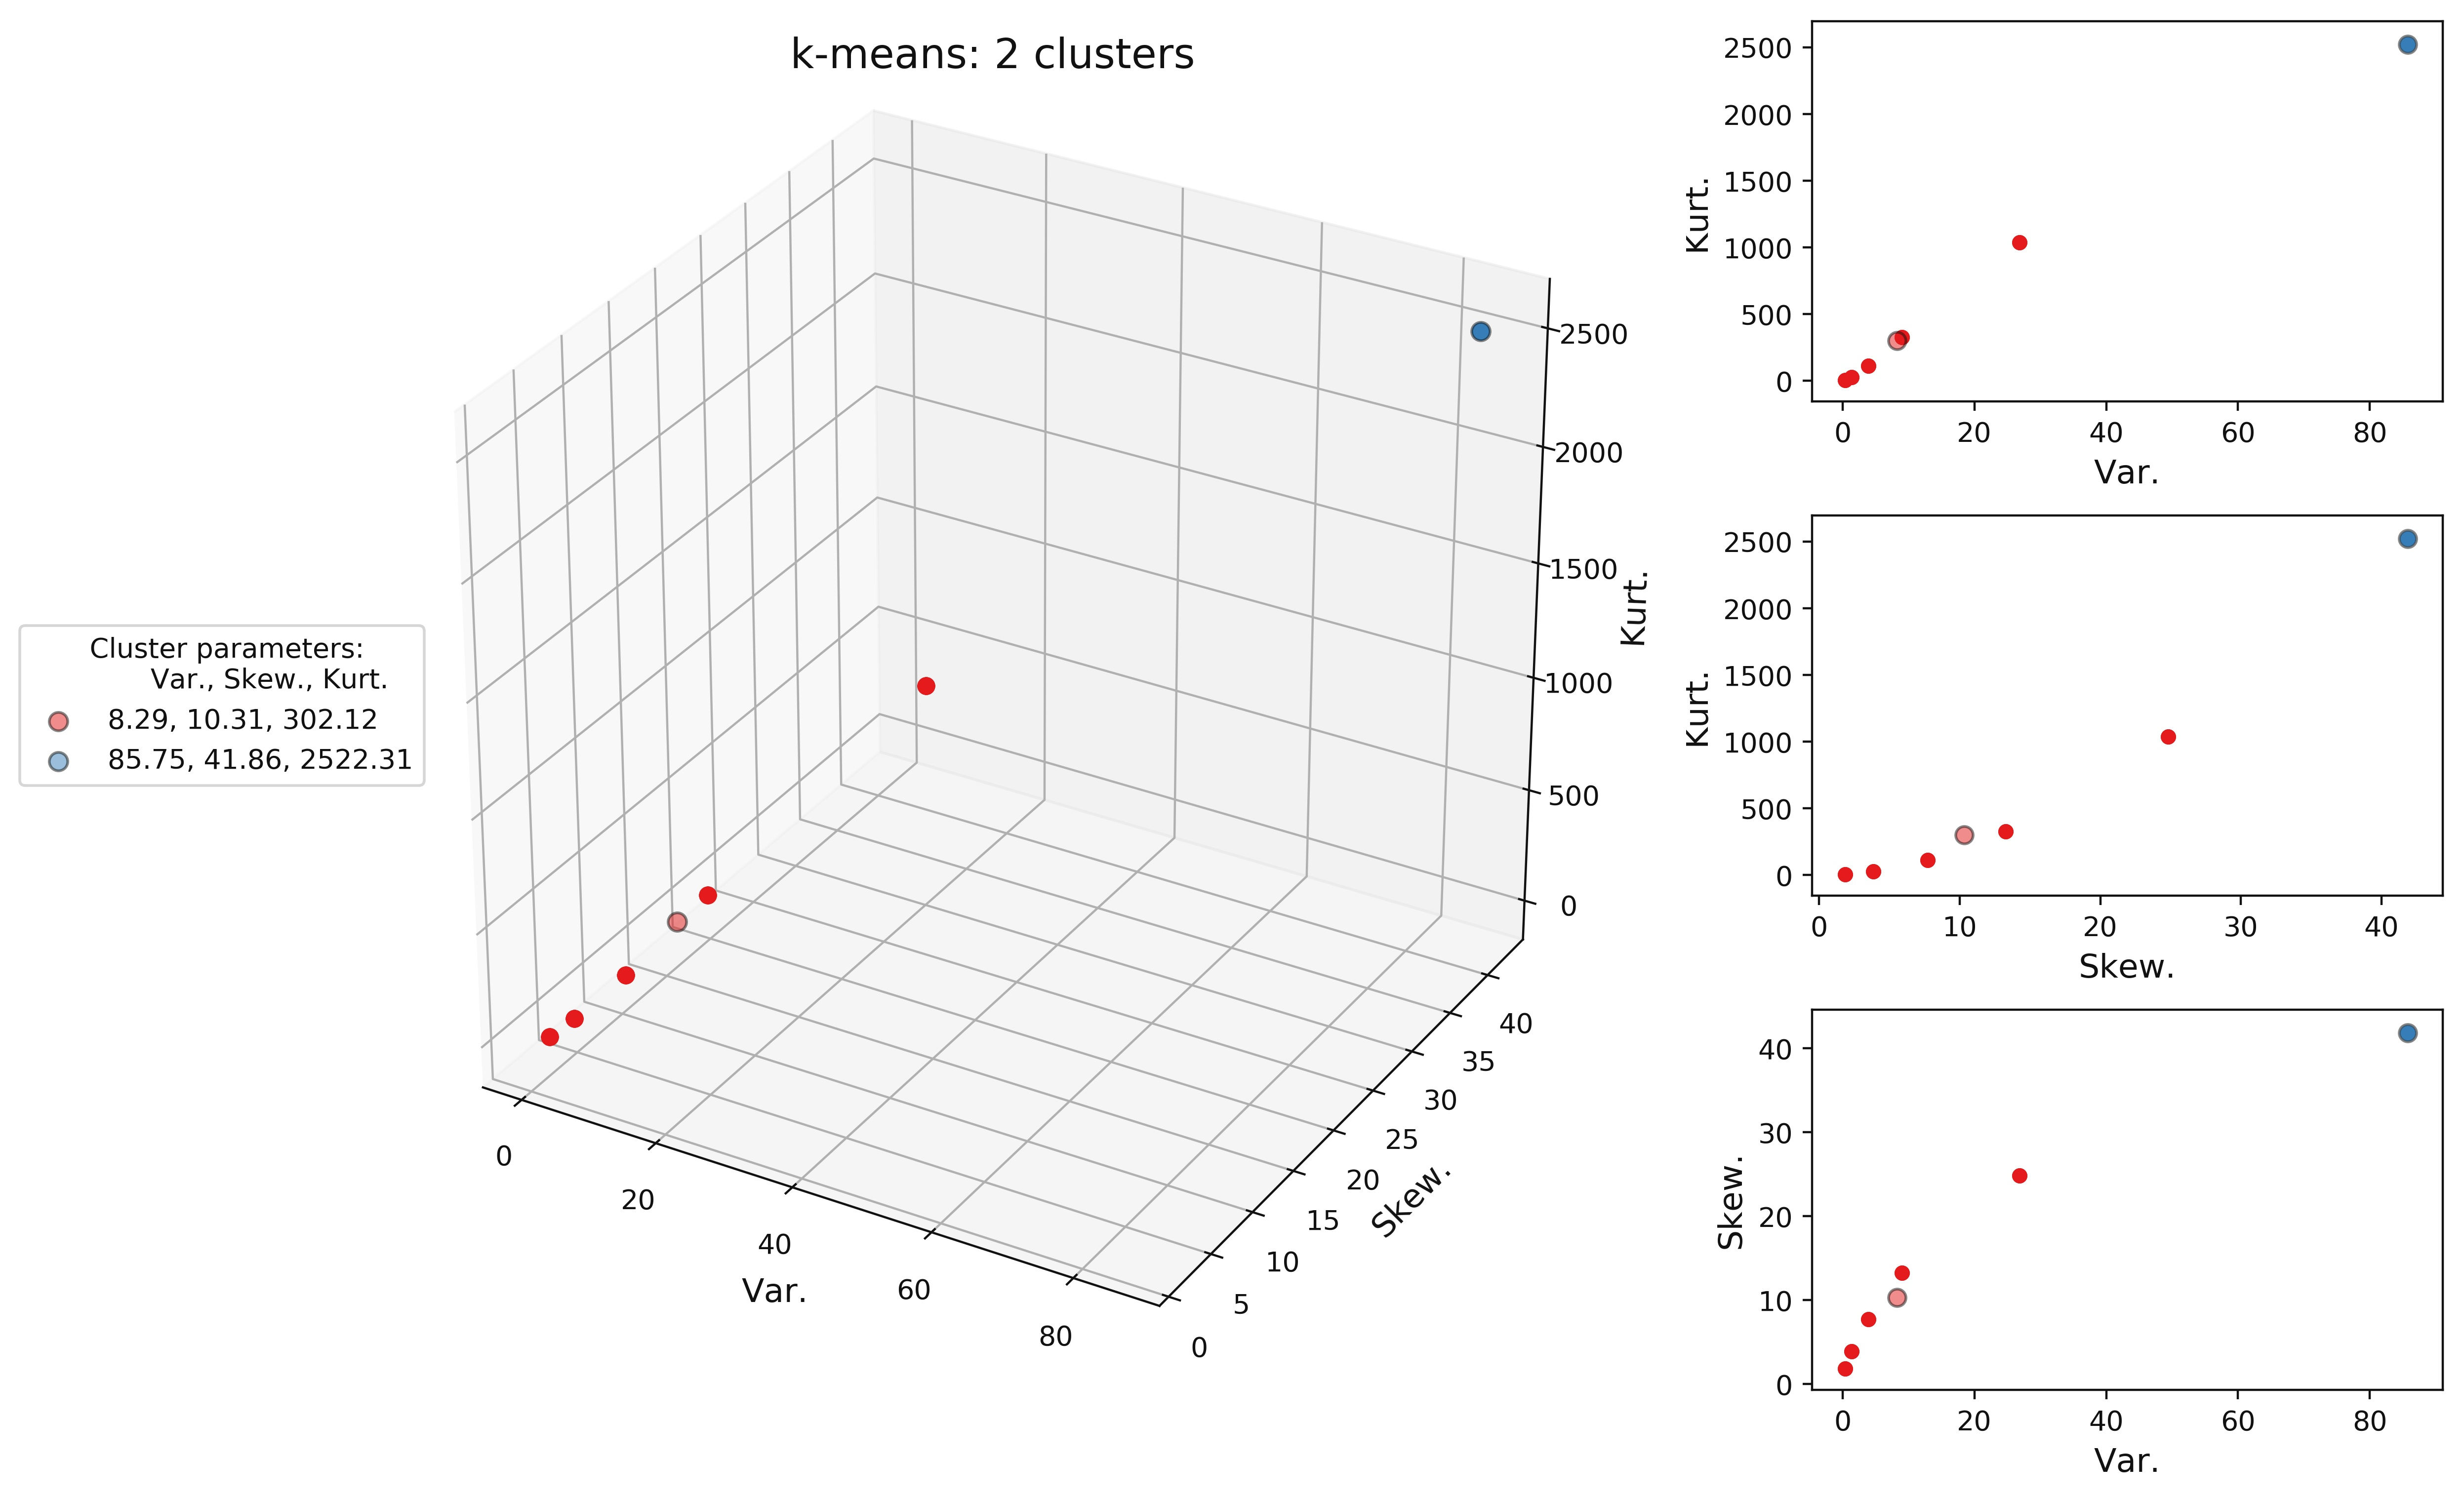
\includegraphics{Figuras/ex3/Exercicio3_cluster_2.jpg}}		
	\end{center}
	\vspace{-2mm}	% acrescentar o espaçamento vertical apropriado entre a borda inferior da figura e a legenda ou a fonte quando não há legenda (o valor pode ser negativo para subir)
	\legenda{Figura 3.3: Técnica kmeans no espaço de parâmetros variância x skewness x kurtosis para todos os sinais da família de sinais pmnoise (endógenos e exógenos). Resultado para número de clusters $n\_c$ = 2.}	% legenda - para deixar sem legenda usar comando \legenda{} (nunca deve-se comentar o comando \legenda)
	\label{ex3_fig3}
	%\FONTE{}	% fonte consultada (elemento obrigatório, mesmo que seja produção do próprio autor)
\end{figure}

\begin{figure}[ht!]
	%\caption{Série e histogramas.}
	\vspace{-3mm}	% acrescentar o espaçamento vertical apropriado entre o título e a borda superior da figura
	\begin{center}
		\resizebox{11cm}{!}{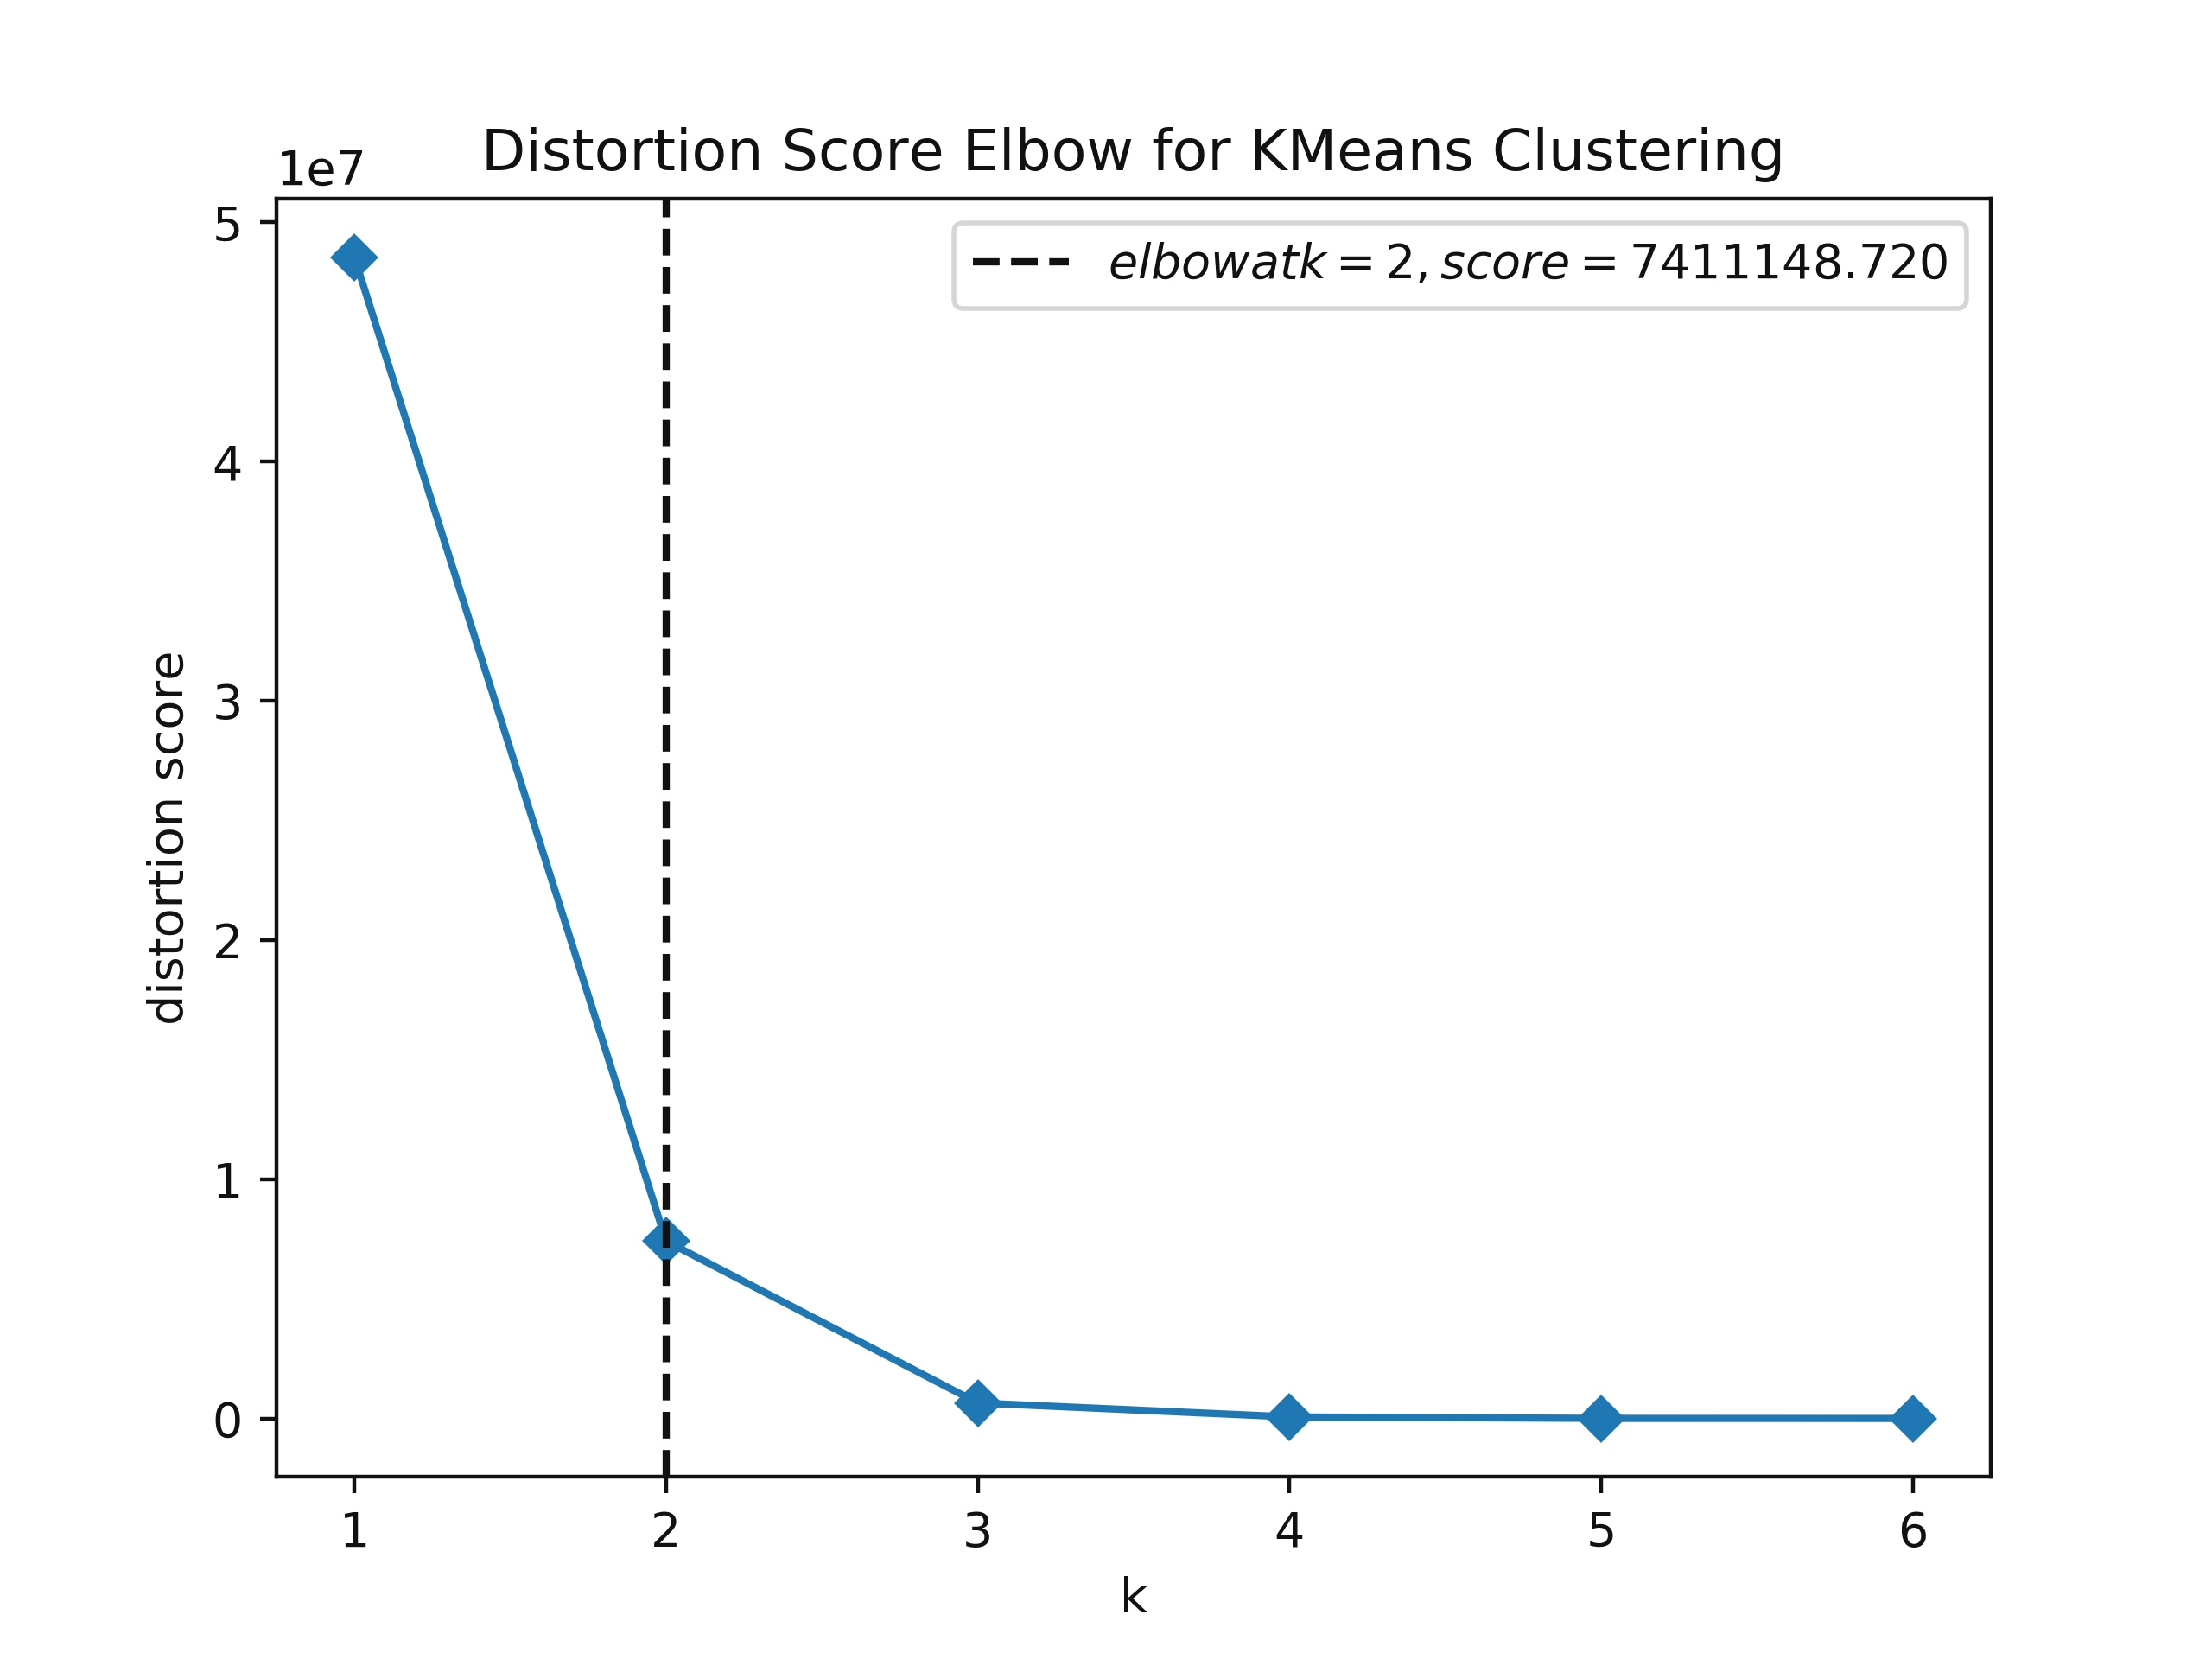
\includegraphics{Figuras/ex3/Exercicio3_elbow_algorithm.jpg}}		
	\end{center}
	\vspace{-3mm}	% acrescentar o espaçamento vertical apropriado entre a borda inferior da figura e a legenda ou a fonte quando não há legenda (o valor pode ser negativo para subir)
	\legenda{Figura 3.4: Resultado do método do cotovelo, mostrando que $n\_c$ = 2 obteve a melhor performance durante o agrupamento da família pmnoise no espaço de parâmetros considerado.}	% legenda - para deixar sem legenda usar comando \legenda{} (nunca deve-se comentar o comando \legenda)
	\label{ex3_fig4}
	%\FONTE{}	% fonte consultada (elemento obrigatório, mesmo que seja produção do próprio autor)
\end{figure}
